\documentclass[11pt]{article}
\usepackage[utf8]{inputenc}
\usepackage[T1]{fontenc}

\usepackage{amsfonts,amsmath,amssymb,graphicx}
\usepackage[portuguese]{babel}
\usepackage{txfonts}
\usepackage[left=2cm,right=3cm,top=3cm,bottom=2cm]{geometry}
\usepackage[dvipsnames]{xcolor}
\usepackage[hidelinks]{hyperref}



\hypersetup{
colorlinks = true,
urlcolor= Blue,
}


%\usepackage[]{}
%\setlength{\parindent}{12pt}
%\setlength{\parskip}{12pt}

\begin{document}
\begin{center}
\huge \sc Curriculum Vitae\\
\Large \sc Junior Rodrigues Ribeiro
\end{center}

\begin{flushright}
\fbox{
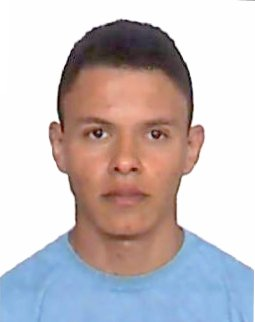
\includegraphics[width=3cm]{Avatar}
}
\end{flushright}
\vspace*{-4.4cm}

\section{Dados pessoais\dotfill\dotfill\dotfill \hfill \ }
\begin{description}
\item[Nome:] Junior Rodrigues Ribeiro.
\item[Celular/WhatsApp:] (16) 98253-4027.
\item[E-mail:] \href{mailto:j5r@outlook.com}{\nolinkurl{j5r@outlook.com}}.
\item[Endereço:] Pq. Arnold Schmidt, São Carlos -- SP.
\item[Escolaridade:] Graduado em Matemática Licenciatura Plena pela UEMS, 2015,\\
\phantom{Escolarid} Mestre em Ciências (Ciências Matemáticas e Computação) pelo ICMC/USP, 2019.\\
\phantom{Escolarid} Doutorando em Ciências (Ciências Matemáticas e Computação) pelo ICMC/USP, 2022.
\end{description}

\section{Objetivos \dotfill}
Minha recente formação em Matemática Computacional me possibilita trabalhar no ramo de tecnologia, uma realização pessoal  que me garantirá novas experiências no mercado. Poderei aprender muito com a empresa e também me desafiar com os problemas tratados. Sou Júnior (além de meu próprio nome), e gostaria de saciar minha vontade de programar,  principalmente quando se tem alguma finalidade prática útil. Toda a experiência obtida me auxiliará na preparação de materiais didáticos para ensino de programação, uma vez que minha formação inicial é Licenciatura, e compartilhar conhecimento é outra coisa de que gosto muito. Ainda não tive a oportunidade de trabalhar com tecnologia em uma empresa ou em grupo, portanto terei bastante coisa interessante a aprender nesse meio.
 
\section{Informações relevantes \dotfill}
\begin{itemize}
\item Idiomas: \\Espanhol --- Básico/Intermediário;\\ Inglês --- Básico/Intermediário;

\item Escritório: Tenho conhecimentos em Microsoft Word, Excel, Power Point e Outlook e suas versões do pacote Libre Office; boas habilidades de escrita e correção ortográfica; conhecimentos de LaTeX.

\item Programação:
\begin{itemize}
\item Formato: Estruturada; Orientada a Objeto (POO);
\item Científica: Matlab; C/C++ (nível básico); Python Numpy, Matplotlib;
\item Web: básico de HTML/CSS; Python BeautifulSoup, Selenium;
\item Dados: Python Pandas, Sqlite3, Shelve, Openpyxl;
\item Desktop: OS, Multiprocessing, Threading.
\item GUI: Tkinter;
\item Versionamento: \href{https://github.com/j5r}{\texttt{GitHub}};
\end{itemize}
No momento estou escolhendo alguns materiais para estudar programação web com Django/Flask, NodeJS, React e React-Native para ter uma noção básica de como as coisas funcionam.  No momento em que eu tiver algum projeto bem estruturado para criar, então consolidarei os conhecimentos com a prática. Todos os que apresentei foram aprendidos de forma autodidata, usando principalmente YouTube e por vezes o StackOverFlow para tirar dúvidas, já que minha formação em Matemática não me ajuda no âmbito de TI, precisando então buscar conhecimento por conta própria.

\item Científico: Já estudei disciplinas de otimização: Programação Linear, Inteira, Não-Linear, Dinâmica. 
Aqui está meu \href{http://lattes.cnpq.br/3866983332299702}{\texttt{CV Lattes}}.

\end{itemize}


\section{Experiências anteriores \dotfill}
\begin{enumerate}
\item ESTAGIÁRIO, REFORÇO DE MATEMÁTICA, \textit{EE Pastor Daniel Berg. Dourados -- MS.} Duração de 8 meses, de abril a novembro de 2012. Atividade: ministrar reforço de matemática nas turmas de sexto a nono anos do ensino fundamental (bolsa de extensão universitária da UEMS).

\item ESTAGIÁRIO, COORDENAÇÃO PEDAGÓGICA. {\it FATEC SENAI Dourados -- MS}. Duração de 2 anos, de agosto de 2013 a agosto de 2015. Atividades: criação e geração de relatórios de desempenho e presença dos alunos para envio às empresas contratantes; agendamento de aulas no sistema integrado; atendimento e acompanhamento de questões diversas relacionadas a alunos; {\it check list} de diários dos professores para arquivamento. 


\item OUTRAS EXPERIÊNCIAS, sem finalidade acadêmica:
\begin{enumerate}
\item  Auxiliar de Garçom (finais de semana), 1 mês (novembro de 2012), pizzaria Mordomos do Rei, Dourados--MS;
\item Auxiliar de Escritório (CLT), 7 meses (dezembro de 2012 a junho de 2013), Toldos Líder, Dourados -- MS;
\item  Serviços Gerais (temporário), 2 meses (junho a julho de 2016), JPP Restaurante Prato Rápido Mineiro, São Carlos -- SP.
\end{enumerate}
\end{enumerate}

\end{document}
